\section{Sensoren}
Bewegungs-, Umgebuns- und Lagesensoren.
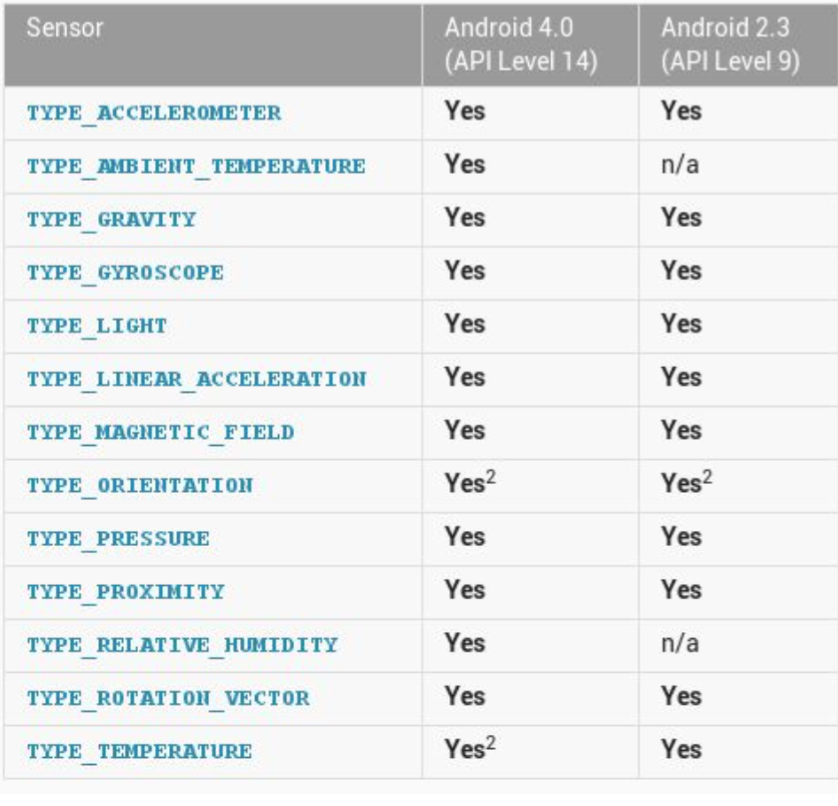
\includegraphics[scale=0.37]{sensors.png} \\
Für die Arbeit mit einem Sensor brauchen wir:
\begin{itemize}
\item \code{SensorManager} als Einstiegspunkt für die Sensoren
\item \code{Sensor} als Repräsentant für einen konkreten Sensor
\item \code{SensorEventListener} um Updates von Sensoren zu registrieren
\item \code{SensorEvent} um die Sensordaten auszulesen
\end{itemize}
Ein Sensor liefert uns nur Rohdaten! Je nach Sensor unterschiedlich zu interpretieren. Sensor Bsp.:
\begin{lstlisting}[language=java]
public class MainActivity extends AppCompatActivity implements SensorEventListener {
   private TextView textView;
   private SensorManager sensorManager;
   private Sensor lightSensor;
   @Override
   protected void onCreate(Bundle savedInstanceState) {
        // ...
        textView = (TextView) findViewById(R.id.textView);
        sensorManager = (SensorManager) getSystemService(Context.SENSOR_SERVICE);
       
        if (mSensorManager.getDefaultSensor(Sensor.TYPE_LIGHT) != null){
          // Success! There's a light sensor.
          lightSensor = sensorManager.getSensorList(Sensor.TYPE_LIGHT).get(0);
        }
        else {
          // Failure! No sensor.
        }
        
   }
   @Override
   protected void onResume() {
       super.onResume();
       //would return true if the sensor is supported and successfully enabled.
       sensorManager.registerListener(this, lightSensor, SensorManager.SENSOR_DELAY_NORMAL);
   }
   @Override
   protected void onPause() {
       super.onPause();
       sensorManager.unregisterListener(this);
   }
   @Override
   public void onSensorChanged(SensorEvent event) {
       textView.setText(String.format("Helligkeit: %.0f", event.values[0]));
   }
}
\end{lstlisting}
\subsection{Dependency Injection}
Oftmals sind Klassen abhängig von anderen Klassen. Beispiel:
\begin{lstlisting}
public class MainViewModel extends ViewModel {
  private final BeersRepository beersRepository;
  private final LikesRepository likesRepository;
  public MainViewModel() {
   beersRepository = new BeersRepository();
   likesRepository = new LikesRepository(); } }
\end{lstlisting}
Beim Testen von MainViewModel werden auch die Repositories instanziert,  welche wiederum eine Abhängigkeit haben (z.B Firestore). Somit wird Unit-Testing von MainViewModel unmöglich. \\
\paragraph{Dependencies von Ausserhalb}
Man könnte natürlich auch den Konstruktor so abändern, dass die Repositories übergeben werden müssen: \code{public MainViewModel(BeersRepository beersRepository, ...)} \\
Noch besser: Interface extrahieren und im Test durch einen Fake/Mock ersetzen. Die Klasse erstellt seine Dependencies also nicht selbst, stattdessen werden diese injiziert (injected). Aber Aufrufer muss sich um Instanzierung kümmern. \\
\paragraph{Dependencies Übergeben}
\textbf{Einfache Lösung:} Konstruktor mit Parametern und final-Attributen. Stellt sicher das Klasse vollständig initialisiert wurde. \\
\textbf{Weniger schön:} Setter Methoden. Entwickler muss acht geben, diese auch alle aufzurufen. \\
\paragraph{DI mit Dagger 2} 
Ein Dependecy-Injection Framework wie Digger 2 übernimmt das Erstellen für uns. Es besteht aus drei grundlegenden Teilen:\\
\textbf{Modul} instanziert unsere Klasse(z.B. Repository) die wir injecten wollen. \textbf{Komponente} fasst Module zusammen und ist zuständig für die Injection. Eine Klasse lässt sich über die Komponenten ihre Abhängigkeiten injecten.
\begin{lstlisting}[language=java]
@Module 
public class BeersRepositoryModule {
  @Provides
  @Singleton
  public BeersRepository getBeersRepository() {
    return new BeersRepository();
  } 
} 
@Singleton 
@Component(modules = {BeersRepositoryModule.class}) 
public interface BeerProComponent {
  void inject(MainActivity activity); 
} 
\end{lstlisting}
\begin{lstlisting}[language=java]
public class Application extends android.app.Application {
   BeerProComponent component;

   public void onCreate() {
     component = DaggerBeerProComponent.builder().build();
   }

   public BeerProComponent getComponent() {  return component;  }
}


public class GadgeothekActivity extends AppCompatActivity {

   @Inject
   BeersRepository beersRepository;

   @Override
   protected void onCreate(Bundle savedInstanceState) {
   ...
   ((Application) getApplication()).getComponent().inject(this);
\end{lstlisting}
Lohnt sich Dependency Injection? \\
Vorteile:
\begin{itemize}
\item Dependencies nicht mehr selbst instanzieren
\item zentrale Konfiguration in Modul und Komponente 
\item einfache Testbarkeit: Modul oder Applikation austauschen
\end{itemize}
Nachteile:
\begin{itemize}
\item Höhere Komplexität, nicht lohnenswert bei kleinen Projekten 
\item Braucht Tests: bei einer Fehlkonfiguration drohen NullPointerException 
\end{itemize}

\subsection{View Injection}
Das Problem ist, dass jede View in der Activity geladen werden muss z.B \code{emailView = findViewById(R.id.email}. Dieser Schritt kann jedoch vereinfacht werden.
\paragraph{Butter Knife}
ButterKnife verwendet ähnliche Implementierung wie Dagger und löst das oben erwähnte Problem.
Kein eigentliches Dependency Injection. A butter knife is like a dagger only infinitely less sharp:
\textbf{Butter Knife Binding}
\begin{lstlisting}[language=java]
class ExampleActivity extends Activity {
  @BindView(R.id.username) EditText username;
  @BindView(R.id.password) EditText password;
  @BindString(R.string.login_error) String loginErrorMessage;
  @OnClick(R.id.submit) 
  void submit() {
    ...   }
  @Override 
  public void onCreate(Bundle savedInstanceState) {
    super.onCreate(savedInstanceState);
    setContentView(R.layout.simple_activity);
    ButterKnife.bind(this);
    ...   } } 
\end{lstlisting}

\subsection{Data Binding}
\begin{itemize}
    \item erspart Tipparbeit
    \item in XML direkt auf Objekte zugreifen (Bsp. \code{onClick})
    \item Optimal: GUI aktualisiert sich selbst, sobald Objekt sich ändert
    \begin{itemize}
        \item XML-Layout als Observer
        \item Einfache Logik (x ? y : z) direkt im XML
    \end{itemize}
\end{itemize}
\textbf{Data Binding Grundlagen}
\begin{lstlisting}[language=java]
public class User {
   public String firstName;
   public String lastName;

   public User(String firstName, String lastName) {
     this.firstName = firstName;
     this.lastName = lastName;
   } }
\end{lstlisting}
\begin{lstlisting}[language=java]
<layout xmlns:android="http://schemas.android.com/apk/res/android">
   <data >
     <variable name="user" type="ch.hsr.mge.User"/>
   </data>
   <RelativeLayout
     ... >

     <TextView android:text="@{user.firstName}" ... />

     <TextView android:text="@{user.lastName}"  ... />
   </RelativeLayout>
</layout>
\end{lstlisting}
Expression Language unterstützt fast alle Java Expressions (Keine Statements Deklarationen, Loops, kein new, this und super)
\begin{lstlisting}[language=java]
android:text="@{String.valueOf(index + 1)}"
android:visibility="@{age < 13 ? View.GONE : View.VISIBLE}"
android:transitionName='@{"image_" + id}'
\end{lstlisting}
\begin{lstlisting}[language=java]
public class MainActivity extends AppCompatActivity {

   @Override
   protected void onCreate(Bundle savedInstanceState) {
     super.onCreate(savedInstanceState);

     ActivityMainBinding binding = 
       DataBindingUtil.setContentView(this, R.layout.activity_main);

     User user = new User("Mirko", "Stocker");
     binding.setUser(user);
   }
}
\end{lstlisting}
\textbf{Binding von Presentern}
\begin{lstlisting}[language=java]
public interface Presenter { 
  void onSaveClick(Task task) 
} 

<layout ...>
  <data>
    <variable name="task" type="ch.hsr.mge.Task" />
    <variable name="presenter" type="ch.hsr.mge.Presenter" />
  </data>
  <LinearLayout ...>
    <Button ...
      android:onClick="@{() -> presenter.onSaveClick(task)}" />
  </LinearLayout> 
</layout> 
\end{lstlisting}
Neben Properties können auch Events gebunden werden
\begin{lstlisting}[language=java]
<Button
   android:text="Save"
   android:onClick="@{controller.onButtonSaveClicked}"/>
   <EditText
   android:text="@{user.lastName}"
   android:addTextChangedListener="@{user.lastNameWatcher}" />
\end{lstlisting}
\textbf{Binding von Listenern}
\begin{lstlisting}[language=xml]
<Button
  android:text="Save"
  android:onClick="@{controller::onButtonSaveClicked}"/>

<EditText
  android:text="@{user.lastName}"
  android:addTextChangedListener="@{user.lastNameWatcher}" />
\end{lstlisting}
\textbf{Automatische Updates}
Was geschieht, wenn sich das gebundene Objekt ändert?
\begin{lstlisting}[language=java]
public class User {
   public String lastName;
   public boolean isDirty;
  
   public TextWatcher lastNameWatcher = new TextWatcher() {
     @Override
     public void beforeTextChanged(CharSequence s, int start, int count, int after) { }

     @Override
     public void onTextChanged(CharSequence s, int start, int before, int count) {
       lastName = s.toString();
     }

     @Override public void afterTextChanged(Editable s) { }
   };
}
\end{lstlisting}
\textbf{Noch mehr Observables}
Um Daten aus gebundenen Objekten in der View zu aktualisieren benötigen wir wieder das Observer-Pattern. \textbf{View} observiert das gebundene Objekt. \textbf{Objekt} ist observable. Um unser Objekt observable zu machen müssen wir \code{ObservableFields} verwenden.
\begin{lstlisting}[language=java]
public class User {
   public ObservableField<String> firstName = new ObservableField<>();
   public ObservableField<String> lastName  = new ObservableField<>();

   public TextWatcher lastNameWatcher = new TextWatcher() {
   ...
      if (!Objects.equals(lastName.get(), s.toString())) {
        lastName.set(s.toString());
      }
   }
};
\end{lstlisting}
\paragraph{Zusammenfassung Data Binding}
Vorteile: \\
- Weniger Code um Daten und Views abzugleichen \\
- Nach Umgewöhnung bessere Lesbarkeit \\
Nachteile: \\
- Aufpassen, dass nicht zu viel Logik ins Layout wandert \\
- Android generiert noch mehr zusätzlichen Code \\
- Code schwieriger zu testen und zu debuggen \\
- Integration mit LiveData-Observables möglich \\

% \subsection{Gradle}

% \begin{lstlisting}
% // build.gradle APP
% apply plugin: 'com.android.application'

% android {
%     compileSdkVersion 26
%     buildToolsVersion '26.0.2'
%     defaultConfig {
%         applicationId "io.teiler.android"
%         minSdkVersion 23
%         targetSdkVersion 26
%         versionCode 1
%         versionName "1.0"
%         testInstrumentationRunner "android.support.test.runner.AndroidJUnitRunner"
%     }
%     buildTypes {
%         release {
%             minifyEnabled false
%             proguardFiles getDefaultProguardFile('proguard-android.txt'), 'proguard-rules.pro'
%         }
%     }
% }

% repositories { jcenter() }
% ext { materialSpinnerVersion = "1.2.1" }
% dependencies {}

% // build.gradle ROOT
% // Top-level build file where you can add configuration options common to all sub-projects/modules.

% buildscript {
%     ext.kotlin_version = '1.1.51'
%     repositories {
%         google()
%         jcenter()
%     }
%     dependencies {
%         classpath 'com.android.tools.build:gradle:3.0.1'
%         classpath ...
%     }
% }

% allprojects {
%     repositories {
%         google()
%         jcenter()
%     }
% }
% \end{lstlisting}

% \subsection{RecyclerView}

% \begin{lstlisting}[language=java]
% public class MyAdapter extends RecyclerView.Adapter < ViewHolder > {
%  private ArrayList < Person > dataset;
%  public MyAdapter(ArrayList < Person > persons) {
%   dataset = persons;
%  }
%  @Override
%  public ViewHolder onCreateViewHolder(ViewGroup parent, int viewType) {
%   LayoutInflater layoutInflater = LayoutInflater.from(parent.getContext());
%   View v = layoutInflater.inflate(R.layout.rowlayout, parent, false);
%   TextView firstName = (TextView) v.findViewById(R.id.firstName);
%   TextView lastName = (TextView) v.findViewById(R.id.lastName);
%   ViewHolder viewHolder = new ViewHolder(v, firstName, lastName);
%   return viewHolder;
%  }
%  @Override
%  public void onBindViewHolder(ViewHolder holder, int position) {
%   final Person person = dataset.get(position);
%   holder.firstName.setText(person.getFirstname());
%   holder.lastName.setText(person.getLastname());
%  }
%  @Override
%  public int getItemCount() {
%   return dataset.size();
%  }
% }
% public class ViewHolder extends RecyclerView.ViewHolder {
%  final TextView firstName;
%  final TextView lastName;
%  public ViewHolder(View v, TextView firstName, TextView lastName) {
%   super(v);
%   this.firstName = firstName;
%   this.lastName = lastName;
%  }
% }
%\end{lstlisting}
